\chapter{Design, Implementering og test}
I det følgende afsnit vil der blive gjort redde for designprocessen i projektforløbet. Her vil de meste essentielle dele for produktet blive beskrevet, mens resten kan findes i dokumentationens afsnit 4-6.


<<<<<<< HEAD
\section{Første iteration} 
=======
<<<<<<< HEAD
\section{Første Iteration}
Målet med første iteration var undersøgelse og valg af converter topologi. Herefter blev der opstillet en ideel simuleringsmodel for converteren, således analyse og simulering kunne sammenholdes. 
=======
\section{Første iteration}
>>>>>>> fa1abab685664999d4f02ab8e16b42e902091617
Første iteration blev hovedsageligt brugt på, at undersøge mulige converter topologier. Her vil flyback converterens funktionalitet blive beskrevet. 
>>>>>>> ae0636983c77876a6412832acac46881f4d92c01

\fxnote{Hvad er målet for denne itearation, og hvad skal som minimum opnås, før næste iteration påbegyndes?}


\subsection{Flyback converter - CCM}
Der blev valgt en flyback converter opereret i CCM, som converter topologi i projektet. En sådan converter deles op i en primær- og en sekundær side. Primærsiden består af transformatorens primærvikling og et switch-element, der typisk er en MOSFET. Sekundærsiden består af transformatorens sekundærvikling en diode, en kondensator og udgangsbelastningen. En oversigt over den ideelle flyback converter er vist på figur~\ref{fig:flyabck_ideal}. 

\begin{figure}[H]
	\centering
	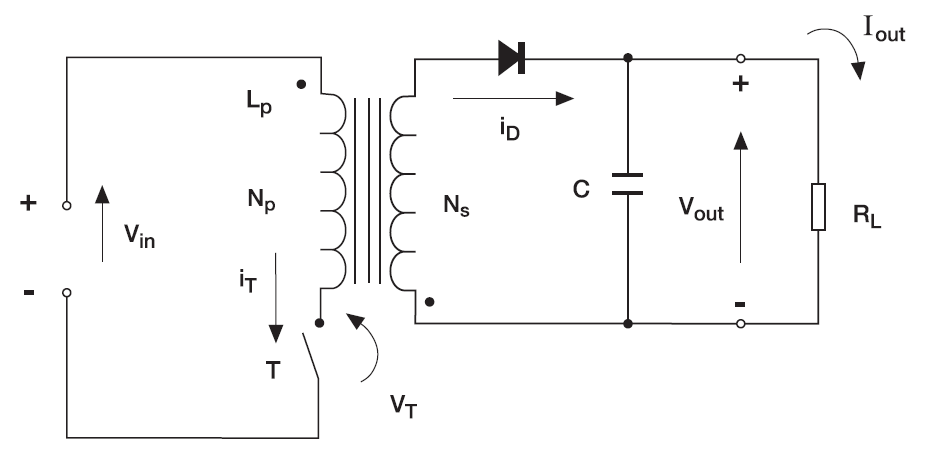
\includegraphics[width=0.7\linewidth]{../Dokumentation/tex/1iteration/billeder/flyback_ideal.png}
	\caption{Ideelt diagram for flyback converteren
		\cite{SMPS-topologies}}
	\label{fig:flyabck_ideal}
\end{figure}

Når MOSFET'en er ON, vil der være en positiv spænding over primærviklingen ved prikenden af viklingen, der er lig indgangsspændingen. Da denne spænding er positiv, vil det få strømmen i viklingen til at stige lineært over den tid MOSFET'en er ON. Strømændringen er bestemt ud fra formlen:
\begin{equation}
V = L \cdot \frac{di}{dt}
\end{equation}

Fordi polariteten af sekundærviklingen er modsat primærviklingen, vil dioden være forspændt i spærreretningen da kondensatoren vil opretholde udgangsspændingen over belastningen. Når dioden ikke kan lede strømmen fra sekundærviklingen, vil transformatoren oplagre energi i kernen når MOSFET'en er ON. Når MOSFET'en går OFF vil strømmen i viklingen ikke kunne skifte momentant. Det vil vende polariteten af transformatoren, så der nu er en positiv spænding diode enden af sekundærviklingen. Nu vil dioden være forspændt i lederetningen, og derfor lede den energi der er blevet oplagret i kernen, i form af en strøm. Den strøm vil nu holde den ønskede udgang, men også oplade kondensatoren, således den kan opretholde udgangsspændingen i næste ON-periode. Da der nu vil være en negativ spænding over sekundærviklingen ift. prikenden af den, vil strømmen i viklingen aftage i løbet af MOSFET'ens OFF periode på baggrund af den førnævnte formel. 

Kurveformen for strømmene i en flyback transformator er vist på figur~\ref{fig:flyabck_ideal_currents}. Her ses det der blev forklaret før. Når MOSFET'en er ON, vil strømmen i primærviklingen rampe op, mens strømmen i sekundærviklingen er 0. Når MOSFET'en er OFF vil strømmen i sekundærviklingen rampe ned fra det niveau primærstrømmen nåede, mens strømmen i primærviklingen nu vil være 0. Niveau-forholdet mellem strømmene i viklingerne, vil blive bestemt af viklingsforholdet i transformatoren. Skal converteren bruges til omsætning af store spændingsændringer fra indgang til udgang, kan dette bruges for at mindske tabet. 

\begin{figure}[H]
	\centering
	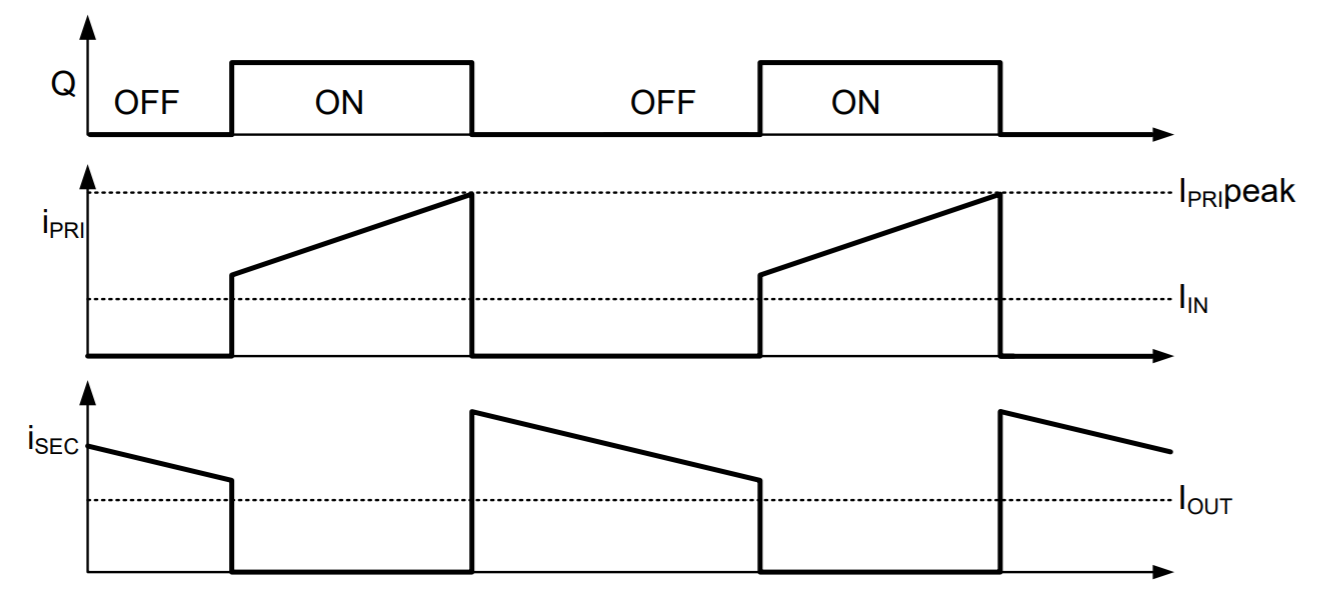
\includegraphics[width=0.7\linewidth]{../Dokumentation/tex/1iteration/billeder/CCM_transformer_current.png}
	\caption{CCM transformator strømme}
	\label{fig:flyabck_ideal_currents}
\end{figure}

selvom transformatoren i helhed opererer i CCM, vil strømmene i individuelt i viklingerne være diskontinuerte. Det betyder peak-strømmene i viklingerne bliver større for at kunne opretholde den ønskede udgangsstrøm. 

\noindent Overføringsfunktionen for flyback converteren i CCM er\cite{SMPS-topologies2}:
\begin{equation*}
	V_{out} = \frac{N_s}{N_p} \cdot \frac{D}{1-D} \cdot V_{in}
\end{equation*}

Da den mindste indgangsspænding og største udgangsspænding converteren skal designes efter næsten er ens, vælges det at tage udgangspunkt i en transformator en et viklingsforhold på 1. Ud fra dette, og intervallet på indgangsspændingen på $26-50V$, kan den maksimale duty-cycle regnes til $D_{maks} = 0.447$ eller $44.7\percent$, og den minimale duty-cycle renes til $0.296$ eller $29.6\percent$.  

Selvinduktionen i transformatorviklingerne bestemmes ud fra den ønskede ripple-strøm i transformatoren og den valgte switch-frekvens. Der er valgt at tage udgangspunkt i en switch-frekvens på $100k\hertz$. Når der er valgt at have et omsætningsforhold på 1, vil denne selvinduktion være gældende for begge viklinger. Selvinduktionen i transformatoren kan designes ud fra følgende formel\cite{flyback-formler}:
\begin{equation*}
	L = \frac{V_{inmin} \cdot D_{min}}{I_{ripple} \cdot f_s}
\end{equation*}

RMS-strømmene i viklingerne har stor betydning for det endelige tab i converteren. Derfor estimeres de i den indledende fase, for at vurdere betydningen af dette. RMS-strømmen i primærviklingen regnes til $3.02A$, og RMS-strømmen i sekundærviklingen regnes til $3.36A$. Begge er regnet ved en indgangsspænding på $26V$. 

Den ideelle converter er simuleret, for kontrol af dens funktionalitet. Figur~\ref{fig:flyabck_ideal_diagram} viser diagrammet for den ideelle converter. Her er der udelukkende fokuseret på transformatoren. Desuden er der indsat en kondensator på $223\micro F$, for at mindske ripple-spændingen på udgangen. Udgangen er blevet simuleret til det forventede $21V$ og $2.5A$, mens RMS-strømmene i transformatorviklingerne stemte overens med det beregnede. 

\begin{figure}[H]
	\centering
	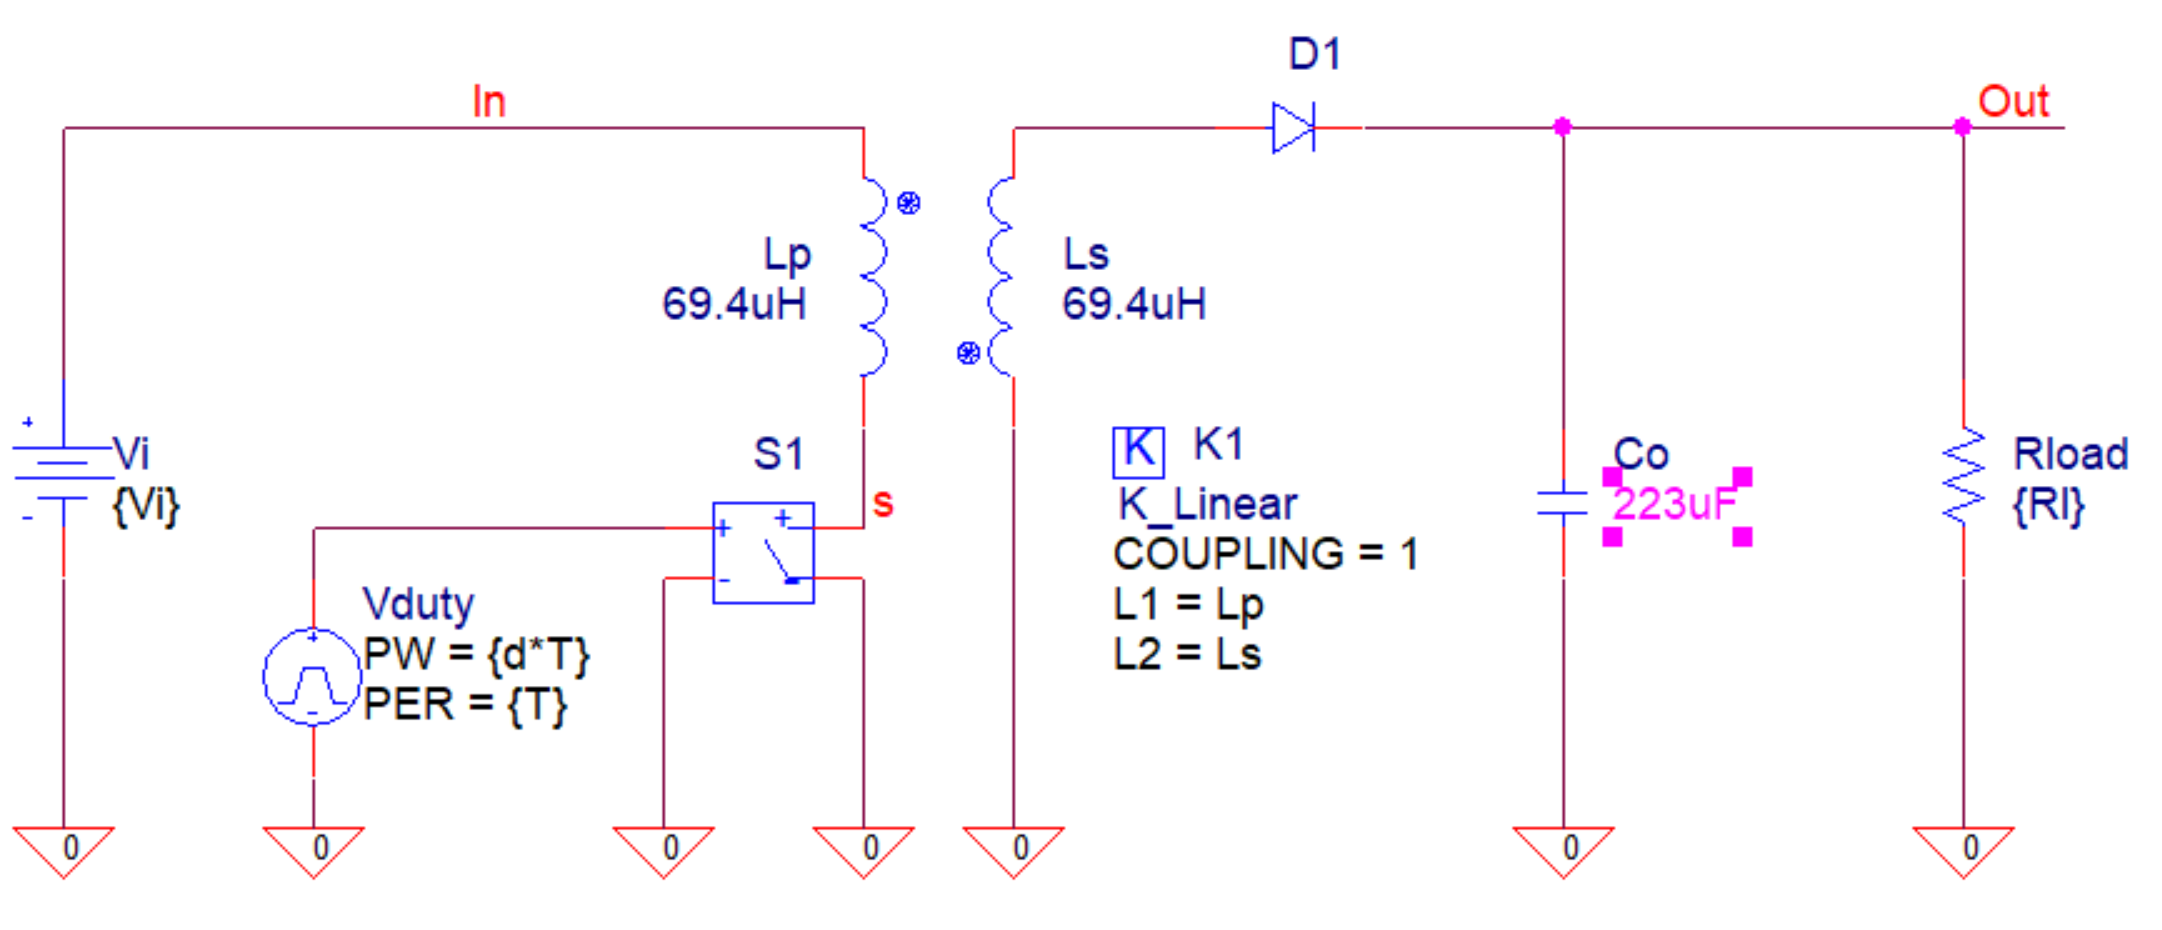
\includegraphics[width=0.7\linewidth]{../Dokumentation/tex/1iteration/billeder/flyback_ideal_diagram.png}
	\caption{Simulering af ideel flyback converter}
	\label{fig:flyabck_ideal_diagram}
\end{figure}

\noindent De præcise beregninger og simuleringer er beskrevet i dokumentationens afsnit 4.4.








\section{Anden iteration}
Målet for 2. iteration var, at indsætte ikke-ideele komponenter ind i modellen fra første iteration. Herudover skulle modellen implementeres for første gang. 
Kravet for at gå videre til 3. iteration var en funktionsdygtig implementeret converter. 
I dette afsnit beskrives hvordan nøglekomponenterne i konverteren er designet, og første implementering af converteren.

\subsection{Transformator}
Flyback converteren fungerer transformatoren lidt anderledes, i forhold til mange andre konstruktioner. Normalt vil der løbe en strøm i både den primære og sekundære vikling på samme tid. På den måde kan energien i transformatoren transformeres direkte fra den primære vikling til den sekundære vikling. Dette er ikke muligt i denne converter typologi, da der kun vil løbe strøm i én vikling ad gangen. Den energi, der skabes i den primære vikling, skal derfor kunne opbevares, indtil der begynder at løbe en strøm i sekundærviklingen. Sker det ikke, går kernen i mætning, hvilket vil sige, at der ikke er en lineær sammenhæng imellem transformatorens H-felt og B-felt.
Dette sikres ved, at indsætte et luftgab i kernen, som øger den magnetiske modstand. Det gør, at kernen kan opbevare mere energi.

I 1. iteration blev det valgt at tage udgangspunkt i en 1:1 transformator. Desuden er det i 2. iteration vigtigst, at få en velfungerende transformator. Derefter kan der senere optimeres på et mere optimalt viklingsforhold, hvis det vurderes nødvendigt. 

Med den estimerede nødvendige induktans beregnet i 1. iteration til $69.43\micro H$, blev energien, der induceres i primærviklingen udregnet til \begin{equation} \label{Primary_energy}
E = \frac{1} {2} \cdot L \cdot {I_{pk}}^2 = 1.083\milli J
\end{equation}

Denne energi skal kunne opbevares i kernen, for at undgå den føromtalte mætning. Hvornår en specifik transformator går i mætning afhænger af selve kernen og dets kernemateriale. Her faldt valget på en RM8 kerne og materialet 3f3, hvilket der er argumenteret for i sektion~\ref{Transana}.
På baggrund af databladet for 3f3, blev luftgabet designet efter at have et maksimalt B felt på $250mT$. Det gav et nødvendigt luftgap på:
\begin{equation} \label{Airgap}
l_g = \frac{L \cdot {I_{pk}}^2 \cdot \micro_0}{B^2 \cdot A_0} = 690.98\micro m
\end{equation}

Dette gav en fornyet induktans på $49\micro H$. Herefter bruges $A_L$ for 3f3 materialet og induktansen til at beregne vindingstallet, som blev udregnet og afrundet til 18 vindinger.
Analysen er herefter holdt op imod simuleringen i p-spice, at sikre at analyse og simulering stemmer overens.
 
Viklingen af transformatoren er sket med en kobbertråd med en diameter på $0.425mm$. Det er en tyndere tråd end analyseret, da der med den beregnede trådtykkelse på $0.45mm$ ikke i praksis kunne vikles 18 vindinger. Det har samtidig øget vindingstallet til 19, for stadig at udnytte hele kernens bredde bedst muligt. Med denne trådtykkelse og vindingstal er hele bredden af kernen på $8.6mm$ fuldt udnyttet. Igen for at fylde kernen ud, er der for både primær- og sekundærsiden viklet 3 viklinger i parallel, for at udnytte højden af kernen. Det giver samlet den tredobbelte højde med 6 viklinger i alt, hvilet ender i en højde $2.867mm$. Viklingen er udført ved skiftevis at vikle en primærvikling og en sekundærvikling. På den måde optimeres koblingen i transformatoren. Imellem viklingerne indsættes tape for at sikre det holdes stramt. På figur~\ref{fig: viklingsoverblik} vises et overblik over viklingerne og dimensionerne. 
\begin{figure}[H]
	\center
	\includegraphics[max width=0.7\linewidth]{../dokumentation/tex/2iteration/billeder/viklingsoverblik.png}
	\caption{Overblik over viklingsantal og tykkelse}
	\label{fig: viklingsoverblik}
\end{figure}
\noindent Med vindingstallet på 19 istedet for 18 er selvinduktionen og dermed strømmene i transformatoren igen korrigeret. Herunder ses den endelig analyserede selvinduktion, ripplestrøm og peakstrøm for den viklede transformator.
\begin{equation} \label{L_2}
L_2 = N^2 \cdot A_L = 57.76\micro H
\end{equation}
\begin{equation} \label{I_ripple_final}
I_{ripple} = \frac{V_{inmin} \cdot D_{max}}{L_2 \cdot f_s} = 2.01A
\end{equation}
\begin{equation} \label{I_pk_final}
I_{pk} = \frac{V_{out} \cdot I_{out}}{V_{inmin} \cdot D_{maks}} + \frac{I_{ripple}}{2} = 5.53A
\end{equation}
Den implementerede transformator ses på figur~\ref{fig: Viklettrans}
\begin{figure}[H]
	\center
	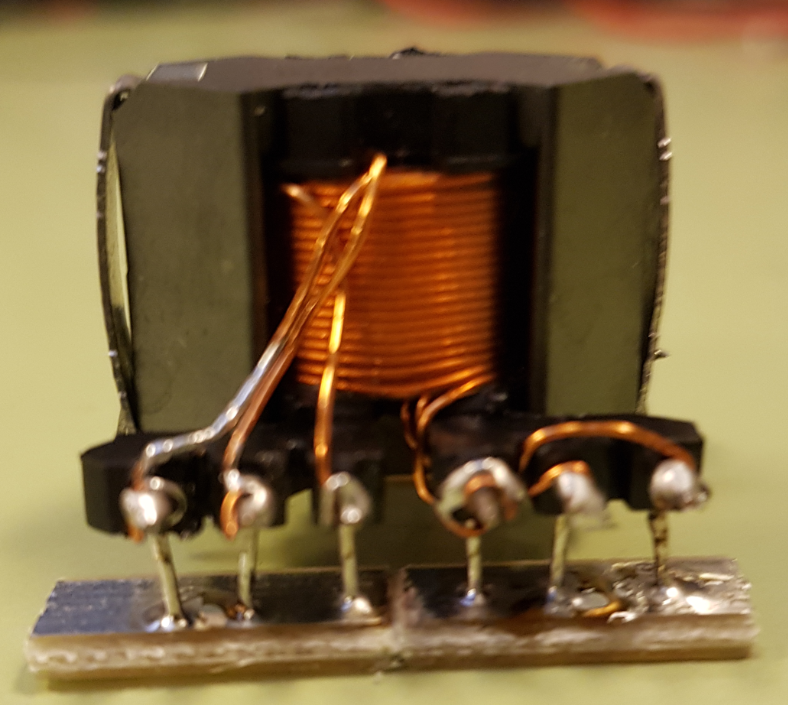
\includegraphics[max width=0.5\linewidth]{../dokumentation/tex/2iteration/billeder/Viklet_transformator.PNG}
	\caption{Viklet transformator}
	\label{fig: Viklettrans}
\end{figure}
\noindent Testen af transformatoren er udført ved at måle selvinduktionen i primær- og sekundærviklingerne samt spredningsselvinduktionen. Det er gjort med en impedansmåler. Her er der benyttet så korte ledninger som muligt samt 4-wire teknikken, for at undgå ekstra induktans fra ledningerne. 

For at måle selvinduktionen i primærviklingen måles henover primærviklingens to sider, mens sekundærviklingen holdes åben. Her laves et frekvenssweep fra $100Hz$ til $1MHz$. Samme fremgangsmåde for sekundærvikligen kan benyttes, men da transformatoren er 1:1, bør det være det samme.
Spredningsselvinduktionen er målt ved måle samme sted, henover primærviklingen, men derudover kortslutte sekundærviklingen. En ideel transformator vil give 0 i sådan en måling. Det betyder, at induktansen målt her, svarer til spredningsselvinduktionen. 

For yderligere forklaring af design, implementering og test af transformatoren henvises til dokumentationen afsnit 5.1, hvor dette er uddybet.
\input{tex/Implementering/2iteration/MOSdiodekon}
\section{Tab}
Dette afsnit omhandler de overvejelser, der er gjort omkring tab i 2. iteration. Her omtales hvilke bidrag, der er taget højde for, til udberegninger af tab for de enkelte komponenter. Udregningerne og yderligere forklaring af disse, kan findes dokumentationen afsnit 5.7.

\subsubsection{Transformator}
Tabet i transformatoren er set som to dele. Et kernetab og et kobbertab. Kernetabet afhænger af  kernematerialet, selvinduktionen og strømmen i viklingerne. Disse bruges til at udregne fluxen i kernen. Med denne værdi og databladskurven for det specifikke tab som funktion af maks flux massefylden, er kernetabet blevet estimeret. 

Kobbertabet kommer af modstanden, der er i kobbertrådene, som er viklet om kernen. Dette indebærer både bidrag fra en DC modstand og en AC modstand. DC modstanden er udregnet ud fra længden og tykkelsen af kobbertrådene. AC modstanden opstår på grund af magnetfeltet kobbertrådene ligger i. AC modstandens del af kobbertabet er der i dette projket ikke valgt at tage højde for.

Det samlede tab for transformatoren er testet, ved at måle temperaturen på kernen efter converteren har været i gang over længere tid. Med en datablads værdi af den termiske modstand for en RM8 kerne er tabet herefter udregnet.   

\subsubsection{MOSFET}
MOSFET'ens tab kan ligeledes deles op i to centrale bidrag; 

conduction tab og switchtab. Conduction tabet kommer af RMS strømmen der løber i MOSFET'ens ON modstand. 

Switchtabet kommer som konsekvens af effekttrekanterne, der opstår, imellem MOSFET'ens ON og OFF perioder. Effekttrekanterne er i dette projekt estimeret ved at udregne dem som arealet af to lige store trekanter. Højden på trekanten er peakaverage strømmen ganget med den maksimale spænding der vil ligge over MOSFET'en. Længden af trekanten fås af den samlede switch-tid i forhold til den samlede switch periode. 

Det samlede tab i MOSFET'en er testet ved at måle temperaturen på kølepladen efter converteren har været i gang over længere tid. Denne temperaturstigning ganget med køle-koefficienten for kølepladen giver tabet. 

\subsubsection{Diode}
Tabet i dioden er udregnet ved, at kigge på spændingsfaldet over dioden ganget udgangsstrømmen. Som nævnt benyttes en schottky diode, og der har derfor ikke været behov for betragtninger af switch-tabet i dioden. 

Tabet for dioden er fundet ved at måle temperaturen af kølepladen ligesom ved MOSFET'en ovenfor.   

\subsubsection{Kondensator}
Med en kendt ESR modstand for kondensatoren, har det været muligt at beregne tabet i denne. Da modstanden er så lille, er tabet dog uden betydning for det samlede tab.

\subsubsection{Current-sence tab}
Tabet i current-sence modstanden er udregnet ved modstandsværdien ganget med RMS strømmen i anden. Strømmen i igennem modstanden er den samme som løber i den primære vikling. 

\subsubsection{Samlet tab}
De ovenstående tab er alle analyseret og simuleret. Derudover er der lavet test af de tab, hvor det var muligt. Resultatet af dette ses i resultatafsnittet \fxnote{indsæt resultatafsnit for tab}.
Det samlede tab for converteren i 2. iteration er i analyse og simulering fundet ved at lægge de fundne tab sammen. I testen er der set på den effekt der sendes ind i converteren og trukket udgangseffekten fra denne.

\section{Tredje iteration}







%%% Første iteration
	% Converter
	
%%% Anden iteration
	% Transformator
	% PWM controller
	% MOSFET, diode og udgangsfilter
	% Regulering
	
%%% Tredje iteration
	% Snubber
	% Switch-tid
	% Udgangsfilter
	% Regulering